\documentclass{standalone}
\usepackage{tikz}
\usepackage{ctex,siunitx}
\usepackage{tkz-euclide}
\usepackage{amsmath}
\usetikzlibrary{patterns, calc}
\usetikzlibrary {decorations.pathmorphing, decorations.pathreplacing, decorations.shapes,}
\begin{document}
\small
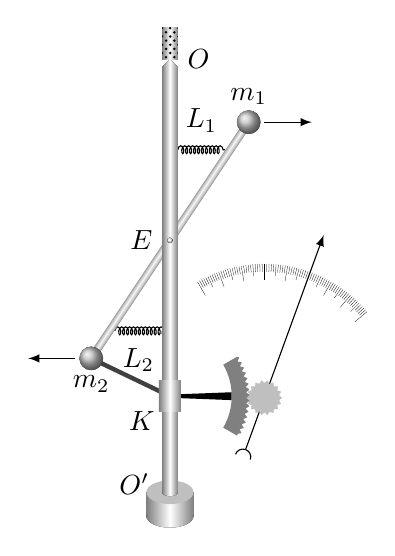
\begin{tikzpicture}[>=latex,scale=1]
  % \useasboundingbox(,)rectangle(,);
  \draw[very thin](0,0)circle(0.05);
  \foreach \x in {110,100,...,40}
  {
    \draw[ultra thin](\x:1.7)--(\x:1.5);
    \foreach \y in {1,2,3,4,6,7,8,9}
    {
      \draw[ultra thin](\x+\y:1.7)--(\x+\y:1.6);
    }
    \draw[ultra thin](\x+5:1.7)--(\x+5:1.55);
  }
  \draw[ultra thin](120:1.7)--(120:1.5);
  \draw[->](-110:0.7)--(70:2.2);
  \draw(-110:0.7)arc(70:-20:0.1);
  \draw(-110:0.7)arc(70:160:0.1);
  \fill[lightgray,even odd rule](0,0)circle(0.2)[rounded corners =0.3mm]
  \foreach \x in {0,20,...,340}
  {
    (\x+5:0.2)--(\x:0.24)--(\x-5:0.2)
    (\x+5:0.2)--(\x+10:0.172554)--(\x+15:0.2)
  };
  \coordinate (C) at ([shift=(-150:1)]-0.35,0.52);
  \coordinate (D) at (C-|-1.2,0);
  \fill([xshift=8mm,yshift=0.05cm]C)--([xshift=8mm,yshift=-0.05cm]C)--([yshift=-0.2mm]D)--([yshift=0.2mm]D);
  \fill[gray, decorate,decoration={snake,segment length=0.7mm,amplitude=0.22mm}](-0.35,0.52)arc(30:-30:1);
  \draw[ultra thick,darkgray](-2.2,0.5)--(D);
  % \draw(-2.2,0.5)--(-2,0.5);
  \draw[decorate,decoration={coil,segment length=0.5mm,amplitude=0.5mm}](-1.9,0.85)--(-1.3,0.85)node[midway,below=1mm]{$L_2$}(-1.1,3.15)--(-0.5,3.15)node[midway,above=1mm]{$L_1$};
  \foreach \x in {90,70,50,30,10}
  {
    \draw[line width={sin(\x)*1mm},gray!\x](-2.2,0.5)--(-0.2,3.5);
  }
  \fill[gray](-0.35,0.52)--++(-150:0.2)arc(30:-30:0.8)--++(-30:0.2);
  
  \fill[left color=gray,right color=gray,middle color=white](-1.2,-1.5)node[above left=2mm]{$O'$}ellipse(0.3 and 0.15);
  \fill[left color=gray,right color=gray,middle color=white](-1.5,-1.5)rectangle(-0.9,-1.2);
  \fill[lightgray](-1.2,-1.2)ellipse(0.3 and 0.15);
  \fill[left color=gray,right color=gray,middle color=white](-1.3,-1.2)--(-1.3,4.2)--(-1.2,4.3)node[right=1mm]{$O$}--(-1.1,4.2)--(-1.1,-1.2)arc(0:-180:0.1 and 0.05);
  \fill[left color=gray,right color=gray,middle color=white](-1.3,4.3)rectangle(-1.1,4.7);
  \fill[pattern=crosshatch dots](-1.3,4.3)rectangle(-1.1,4.7);
  \fill[ball color=lightgray](-2.2,0.5)circle(0.15)node[below=1mm]{$m_2$};
  \fill[ball color=lightgray](-0.2,3.5)circle(0.15)node[above=1mm]{$m_1$};
  \fill[ball color=white](-1.2,2)circle(1pt)node[left=1mm]{$E$};
  \draw[thin,->](0,3.5)--++(0.6,0);
  \draw[thin,->](-2.4,0.5)--++(-0.6,0);
  \fill[left color=gray,right color=gray,middle color=white]([xshift=-1.4mm,yshift=2mm]D)rectangle([xshift=1.4mm,yshift=-2mm]D);
  \node at (D)[below left=1mm]{$K$};
\end{tikzpicture}
\end{document}